\documentclass[11pt,a4paper]{article}
\usepackage{tikz}             
\usepackage{xeCJK}  
\usepackage[fontset=macnew]{ctex}
\usepackage{geometry}
\usepackage{amsmath}
\usepackage{amssymb}
\usepackage{graphicx}
\usepackage{minted}
\geometry{left=2.54cm,right=2.54cm,top=3.18cm,bottom=3.18cm}
\usepackage{pgfplots} % package used to implement the plot
\usepackage{pgf-pie}
\pgfplotsset{width=6.5cm, compat=1.6}
\usepackage{indentfirst}
\usetikzlibrary{shapes,arrows}
\begin{document}
\begin{center}
	\textbf{\Large 数学建模笔记}\\
	\vspace{5pt}
	\vspace{20pt}
	\textbf{龚舒凯 2022202790}\\
	\vspace{5pt}
\end{center}
\section{数学建模思想}
\subsection{灵敏度分析}
\indent\setlength{\parindent}{2em}在数学建模的所有变量里,有些变量是较为可靠的(比如养猪模型:猪的初重量$m_1$、每斤的价格$p_0$等等),但有些变量不确定(比如养猪模型:猪的生长速率$r$),这时候,可以把不确定的变量拎出来,选择不同的$r$算出结果(或者干脆把$r$当成未知量解一解),观察参数的敏感性(比如说$r$的敏感性)。\\
\indent\setlength{\parindent}{2em}怎么描述灵敏性数据呢,还是以养猪为例,可以说成$r$的10$\%$下降造成了出售金额$P$的26$\%$。用数学公式说,$P$的相对改变量为$\dfrac{\Delta P}{P}$,$r$的相对改变量为$\dfrac{\Delta r}{r}$,那么$P$对$r$的灵敏度为:
\begin{equation*}
\lim\limits_{r \to 0}\dfrac{\Delta P / P}{\Delta x/x}=\dfrac{\mathrm{d}x}{\mathrm{d}r}\cdot \dfrac{r}{x}
\end{equation*}
\subsection{鲁棒性分析}
\indent\setlength{\parindent}{2em}鲁棒性指的是模型不完全精确但导出的结果大差不差。

\section{微分方程模型}
\subsection{Logistic曲线}
生物的生长过程经历发生、发展到成熟三个阶段,在三个阶段生物的生长速度是不一样的,例如南瓜的重量增长速度,在第一阶段增长的较慢,在发展时期则突然加快,而到了成熟期又趋减慢,形成一条 S 形曲线,这就是有名的 Logistic曲线(生长曲线),很多事物,如技术和产品发展进程都有类似的发展过程,因此 Logistic 曲线在预测中有相当广泛的应用。\\
Logistic曲线的数学模型是:\\
\begin{equation*}
	\dfrac{\mathrm{d}y}{\mathrm{d}t}=ry(1-\dfrac{y}{L})
\end{equation*}
其中$y$为预测值,$L$为$y$的极限值,$r>0$为增长率常数。解此微分方程模型得到:
\begin{equation*}
	y=\dfrac{L}{1+ce^{-rt}}
\end{equation*}
我们记Logistic曲线的一般形式为
\begin{equation*}
	y=\dfrac{L}{K+ab^{t}}
\end{equation*}
在检验能否使用Logistic曲线时,我们观察$\dfrac{\dfrac{1}{y_{t+1}}-\dfrac{1}{y_t}}{\dfrac{1}{y_t}-\dfrac{1}{y_{t-1}}}$是否接近常数$b$。\\
可以通过这样的公式来估计参数:记\\
\begin{equation*}
S_1=\sum\limits_{t=1}^{m}\dfrac{1}{y_t},\quad S_2=\sum\limits_{t=m+1}^{2m}\dfrac{1}{y_t},\quad S_3=\sum\limits_{t=2m+1}^{3m}\dfrac{1}{y_t}
\end{equation*}
\begin{equation*}
	\begin{cases}
	b=(\dfrac{S_3-S_2}{S_2-S_1})^{\frac{1}{m}}\\
	a=(S_2-S_1)\dfrac{b-1}{b(b^m-1)^2}\\
	K=\dfrac{1}{m}(S_1-\dfrac{ab(b^m-1)}{b-1})
	\end{cases}
\end{equation*}
\subsection{Lotka-Volterra 猎食者-猎物模型}
\indent\setlength{\parindent}{2em}猎物的种群数量$U(t)$和捕食者的种群数量$V(t)$随时间$t$的变化由如下的Lokta-Volterra方程给出:
\begin{equation*}
	\begin{cases}
	\dfrac{\mathrm{d}U}{\mathrm{d}t}=\alpha U-\gamma UV\\
	\\
	\dfrac{\mathrm{d}V}{\mathrm{d}t}=-\beta V+e\gamma UV\\
	\end{cases}
\end{equation*}
\indent\setlength{\parindent}{2em}方程右边的第一项给出的是各种群自身在自然环境下的变化趋势,而第二项描述的是猎物被猎食者捕杀导致的变化。具体而言,可以把$\alpha$看作猎物的自然增长率,即它们的自然出生率和自然死亡率之间的差。在此我们假定猎物生存所需的资源总是充沛的,如果不存在天敌,则它们的种群可以不断繁衍,其数量呈指数增长。而对于猎食者而言,如果没有了猎物,它们就会因为缺少食物资源而饿死,自然增长率为负,所以方程中的$\beta$可以想象成它们的自然死亡率。\\
\indent\setlength{\parindent}{2em}另一方面,如果考虑猎物本身受到捕食,猎物的种群数量会减少。$\gamma$可以视作猎物在单位时间内被猎食者捕获的比例,所以在$\mathrm{d}t$间隔内,被捕获的猎物总数为$\gamma \mathrm{d}t \cdot UV$,可以对应于方程右边的第二项。猎食者有了食物填饱肚子,就有机会繁衍它们的后代。一般猎食者总是需要吃上好几顿饱的,才有机会养育出一个新生宝宝,所以这里会有一个捕获猎物数量和新生小猎食者数量之间的换算关系,方程出现的因子$e$就是这样一个转换系数。\\


\section{概率模型}
\subsection{离散概率模型}
首先回顾一下期望:$E(X)=\sum x_i p_i$,$p_i$表明了随机变量$X$的分布。\\
在建模的时候,首先要假设每个事件发生的概率$p$,以及随机变量(比如:发生随机事件A要付1000元,发生随机事件B要付2000元),然后算一算期望,这大概是一个关于某个变量的函数,然后求其最值。\\
\indent\setlength{\parindent}{2em}根据前面的公式也可以算算它关于某个变量的敏感度。\\
\subsection{连续概率模型}
在连续概率模型中,描述$X$的概率结构的是分布函数$F(x)=P(X)$,密度函数$F'(x)=f(x)$,那么对任意$a<b$有:
\begin{equation*}
P(a<x<b)=F(b)-F(a)=\int_{a}^{b}f(x)\mathrm{d}x
\end{equation*}
这个式子对意思是密度曲线下面的面积给出了概率,从这里出发,$X$的期望可以表达为:
\begin{equation*}
E(X)=\int _{-\infty}^{+\infty}xf(x)\mathrm{d}x
\end{equation*}

\subsection{蒙特卡洛模拟}

\section{规划类问题}
\subsection{多变量最优化}
\indent\setlength{\parindent}{2em}比如通过建模算出来一个模型$y=f(x_1,...,x_n)$,算$y$的极值,那么可以对$y$求偏导:
\begin{equation*}
	\frac{\partial f}{\partial x_i} f(x_1,...x_n)=0
\end{equation*}
这样会得到$n$个方程组,联立求解出来$x_1,...x_n$即可。一般情况下用MATLAB就能实现。\\
\indent\setlength{\parindent}{2em}再提一句,在做多变量最优化的灵敏分析时,可以选择一个变量(比如$y=f(x_1,...,x_n)$这个多项式中某一个系数为$a$)然后再求偏导。这样又可以画出来一个关于$a$的「极值-$a$」函数图像。\\
\indent\setlength{\parindent}{2em}多变量最优化难一点的有两种情况:多个等式约束与多个不等式约束。先说多个等式约束。\\
\indent\setlength{\parindent}{2em}对于多个等式约束条件:
\begin{equation*}
	g_i(x_1,x_2,...x_n)=c_i, (i=1,2...k)
\end{equation*}
目标是要在$\mathrm{R}^n$上求其最大值/最小值。我们要做的就是解方程:\\
\begin{equation*}
	\begin{cases}
		\frac{\partial f}{\partial x_1}=\lambda_1\frac{\partial g_1}{\partial x_1}+...+\lambda_k\frac{\partial g_k}{\partial x_1}\\
		...\\
		\frac{\partial f}{\partial x_n}=\lambda_1\frac{\partial g_1}{\partial x_n}+...+\lambda_k\frac{\partial g_k}{\partial x_n}\\
		g_1(x_1,...,x_n)=c_1\\
		...\\
		g_k(x_1,...,x_n)=c_k\\
	\end{cases}
\end{equation*}
这个方程的解告诉我们极值点在某个解向量$(\xi_1,...,\xi_ n)$取到,把它带入目标函数$f(x_1,...,x_n)$就能得到$f$在这么多等式约束条件下的最值。\\
\subsection{0-1整数规划}
0-1整数规划的特别之处就是引入了一组决策变量$x_1,x_2,...,x_n\in (0,1)$,举一个例子:有$m$台机器,$n$个工件,第$i$台机器的可用工时数为$b_i$,第$i$台机器完成第$j$件工件所需要的工时数为$a_{ij}$,费用为$c_{ij}$,那么如何最优指派机器生产?\\
引入决策变量$x_{ij}=\begin{cases}
1 & \mathrm{Machine}\ i \ \mathrm{Process \ Workpiece} \ j \\
0 & \mathrm{Not-process}\\
\end{cases}$
那么这个指派问题可以表示成下面的整数规划:
\begin{equation*}
	\min\limits_{x} \sum_{i=1}^{m} \sum_{j=1}^{n} c_{ij}x_{ij} 
\end{equation*}
s.t.\\
\begin{equation*}
	\begin{cases}
	 \sum_{j=1}^{n} a_{ij}x_{ij} \le b_i \ (i=1,...,m) \\
	 \sum_{i=1}^{m}x_{ij}=1 \ (j=1,...n) \\
	 x_{ij}\in \{0,1\} \\
	\end{cases}
\end{equation*}
约束条件第一条告诉我们的是,对于每个机器$i$,其加工工时不能超过$b_i$。第二条告诉我们,对于每个工件$j$,仅有一个机器去加工它,至于是哪一个则由决策变量$x_{ij}$决定。第三条就是决策变量的取值,反映「要么选这个机器,要么不选」。
\subsection{目标规划}
\indent\setlength{\parindent}{2em}多变量线性规划下的最优解在现实中不一定能达到,于是人们退而求其次选择“尽量满意的方案”,这时候就要引入目标规划。在目标规划中,除了引入$x_1,...,x_n$外,还引入偏差变量$d_i^+$和$d_i^-$。\\
\indent\setlength{\parindent}{2em}$d_i^+$是正偏差变量,表示第$i$个目标的实际值超出目标值的部分;$d_i^-$是负偏差变量,表示第$i$个目标的实际值不足目标值的差距。对应地,常见目标规划的达成函数有:\\
(1)要求恰好达到目标值,即正负偏差量都要尽可能小,就构造目标函数:$\min z=d_i^+ + d_i^-$\\
(2)要求不超过目标值的,即允许达不到目标值,但即使超过也要越小越好,就构造目标函数:$\min z=d_i^+$\\
(3)要求超过目标值的,即允许超不过目标值,但即使不够,差距也要越小越好的,就构造目标函数:$\min z= d_i^-$\\
综合上面的三种情况,就可以得出总的目标函数:
\begin{equation*}
\min z= \sum_{i,j} (d_i^+ + d_j^-)
\end{equation*}
除了考虑偏差变量之外,在实现多个目标时也有轻重缓急。这里可以设置\textbf{优先因子},比如说先保证$p_1$级别目标的实现,实现了$p_1$级别的再考虑$p_2$级别的目标,以此类推。\\
\newpage
看一个例子:对于一家工厂,已知其在一个周期内有效工时为1400小时,下面是产能、市场需求与利润表:
\begin{table}[h]
	\centering
	\begin{tabular}{cccc}
		\hline
		机床种类& 平均生产一台耗时(小时)  & 一个周期内市场需求量(台) & 利润(元) \\
		\hline
		A & 20 &60 &300\\
		B & 10 &100 &120  \\
		\hline
	\end{tabular}
\end{table}

\noindent 且工厂有三个目标:\\
第一目标:尽量完成本周期的利润指标24000元;\\
第二目标:生产量不超过最大销售量;\\
第三目标:用工总时数最好不超过1400小时,不得已时,超过量越小越好;\\
求利润最大的生产计划。\\

\noindent 第一步:我们令$x_1,x_2$为生产$A,B$的台数,并确定偏差变量。(1)利润指标方面的偏差变量$d_1$(2)生产A的偏差变量$d_2$和生产B的偏差变量$d_3$(3)用工时长的偏差变量$d_4$。
第二部:确定目标函数。第一是利润指标:$p_1d_1^-$(就算少也不能少太多);\\
第二是A的生产量:$2.5p_2d_2^+$(两方面:A更重要,因为它的利润是B的2.5倍,且A就算生产多了也不能多太多)\\
第三是B的生产量:$p_2d_3^+$(B就算生产多了也不能多太多)\\
第四是用工时长:$p_3d_4^+$(用工市场就算多了也不能多太多)\\
因此目标函数是:$\min z= p_1d_1^-+2.5p_2d_2^++p_2d_3^++p_3d_4^+$,接着补齐约束条件即可:
\begin{equation*}
	\begin{cases}
	300x_1+120x_2+(d_1^- - d_1^+)=24000\\
	x_1+(d_2^- - d_2^+)=60\\
	x_2+(d_3^- - d_3^+)=100\\
	20x_1+10x_2+(d_4^- - d_4^+)=1400\\
	x_1,x_2,d_i^-,d_i^+>0\\
	\end{cases}
\end{equation*}
\subsection{非线性规划,动态规划与现代优化算法}
这一部分不是太重点的问题,且可能非常复杂。
可能会用到:遗传算法
包括单目标与多目标规划。
\section{评价体系的建立}
\subsection{权重确定方法:层次分析法(Analytic Hierarchy Process)}
层次分析法在需要主观决策/经验判断的方面较为有效,其作用一般有二:
(1)给指标制定权重:一个时间的因素有$n$个,AHP可以在便无需收集数据的情况下给指标制定权重\\
(2)量化方案选择:根据(1)制定的权重给各个方案打分,从而获得最优方案\\
\indent\setlength{\parindent}{2em}\textbf{需要强调的是,层次分析法仍然是非常主观的(体现在判断矩阵那一步),一致性检验只能告诉你是否自相矛盾的太离谱。}
\textbf{第一步:\textbf{构建层次评价模型:}}a.目标层(最优旅游地选择)b.准则层(景色、费用、居住、饮食、旅途等)c.方案层(北京、上海、广州等)\\
\textbf{第二步:\textbf{构造判断矩阵:}}根据Saaty的1-9标度方法给出,以下为标准:
\begin{table}[h]
	\centering
	\begin{tabular}{cccc}
		\hline
		标度& 含义 \\
		\hline
		1& 两个元素相比,具有同等的重要性\\
		3& 两个元素相比,前者比后者稍重要\\
		5& 两个元素相比,前者比后者明显重要\\
		7& 两个元素相比,前者比后者及其重要\\
		9& 两个元素相比,前者比后者强烈重要\\
		2,4,6,8&上述相邻判断的中间值\\
		1~9的倒数&相应两因素交换次序比较的重要性\\
		\hline
	\end{tabular}
\end{table}
填写判断矩阵时,左边的列为「前者」,上边的行为「后者」。且由上面的定义容易看出,对于判断矩阵$\begin{bmatrix}
a_{11}&a_{12}&...&a_{1n}\\
...&...&...&...\\
a_{n1}&a_{n2}&...&a_{nn}\\
\end{bmatrix}$,有如下成立:\\
(1)$a_{ij}>0$\\
(2)$a_{ij}=\dfrac{1}{a_{ji}}$\\
(3)$a_{ii}=1$\\
\textbf{第三步:\textbf{层次单排序与一致性检验}}\\
\indent\setlength{\parindent}{2em}具体的计算方法不需要掌握,直接使用SPSSPro即可(https://www.spsspro.com/?utm$\_$source=zhihu)。简单介绍一下流程:(1)方根法计算权重\\
(2)获得权重矩阵后计算最大特征根\\
(3)根据最大特征根算出CI值\\
(4)根据CI、RI值求解CR值,判断一致性是否通过。CR<0.1则通过,否则不通过。不通过的原因是填写判断矩阵时出现了逻辑错误。(比如「北京>上海,上海>广州,广州>北京」就是一个逻辑错误)\\
\textbf{第四步:\textbf{层次多排序与一致性检验}}\\
\indent\setlength{\parindent}{2em}第三步只告诉了我们权重,我们的最终目标是对北京、上海、广州进行打分。在SPSSPro上使用AHP专业版即可。简单介绍一下流程:\\
(1)关于准则层的每一个要素(景色、费用...一个个做过去)填写判断矩阵,获取方案层在准则层每一个元素上的得分(比如北京在景色上的得分)\\
(2)计算得分(比如说北京的得分=北京景色得分*景色权重+北京费用得分*费用权重+北京居住评分*居住权重+北京饮食得分*饮食权重+北京旅途得分*旅途权重)\\
(3)根据得分由大至小评价方案\\
\indent\setlength{\parindent}{2em}\textbf{当然,第四步也可以不用做,因为有时层次分析法就是为了去确定权重的,至于最后的方案评价也可以采用别的方法}。
\subsection{权重确定方法:熵权法(Entropy Weight Model)}
\indent\setlength{\parindent}{2em}熵权法比层次分析法更为可观:层次分析法通过「填写判断矩阵」的方式得到权重主观性太强,而熵权法完全从客观数据出发得到权重。但是,熵权法只从数据出发,不考虑问题的实际背景,确定权重时就可能出现与常识相悖的情况。因此,层次分析法和熵权法应该灵活使用。\\
EWM的原理是:指标的变异程度(方差)越小,所反映的信息量也越少(同时信息熵越大),其对应的权值也应该越低。直白一点来说: 越可能发生的事信息熵越大,信息量越少,权值也越低。\\
\indent\setlength{\parindent}{2em}在EWM中,首先要明确哪些是正向指标,哪些是负向指标。其中正向指标是数值越大越好(GDP),负向指标是数值越小越好(失业率)。有的时候一些指标呈现出了区间的形式(比如pH值),这时候要将其转化为正向或负向指标。举个例子:如果定义6.3--7.3是对生物无害的pH值,偏离该区间呈线性的伤害,那么衡量pH=8.3对该生物的危害值可以计算为:$8.3-7.3=1$。\\
实际上,熵权法也可以通过SPSSPro轻易计算得出,下面先阐述步骤:\\
(1)首先对$n$个要评价对象,$m$个评价指标,构建原始矩阵$O_{ij}$\\
(2)对原始矩阵$O_{ij}$进行规范化得到规范化矩阵$N_{ij}$,先去量纲,常常再使用极差法,其中:\\
对正向指标,$n_{ij}=\dfrac{{o_{ij}-\min(o_{j})}}{{\max(o_{j})-\min(o_{j})}}$\\
对负向指标,$n_{ij}=\dfrac{\max(o_{j})-{o_{ij}}}{{\max(o_{j})-\min(o_{j})}}$\\
(3)对规范化矩阵$N_{ij}$,计算第$j$个评价指标下第$i$个样本值占该指标的比重:
\begin{equation*}
	\rho_{ij}=\dfrac{x_{ij}}{\sum_{i=1}^{m}x_{ij}} \ (i=1,2,...,n;\ j=1,2,...,m)
\end{equation*}
(4)计算第$j$个指标的熵:
\begin{equation*}
	e_j=-\dfrac{1}{\ln n}\sum_{i=1}^{n}\rho_{ij}\ln\rho_{ij}
\end{equation*}
(5)计算第$j$个指标的差异系数:$d_j=1-e_j$\\
(6)计算第$j$个指标的权重:
\begin{equation*}
	\omega_j=\dfrac{d_j}{\sum_{i=1}^{m}d_j}\ (j=1,2,...,m)
\end{equation*}
这样就得到了每一个指标的权重$\omega_i$。
\subsection{主成分分析法}
\newpage
\subsection{评价模型:TOPSIS模型}
TOPSIS即优劣解距离法。由于我们可以根据给定的数据,构造出一个所有方案组成的系统中的理想最优解和最劣解。TOPSIS做的就是通过一定的计算,评价系统中任何一个方案距离理想最优解和最劣解的综合距离。如果一个方案离理想最优解更近,离最劣解更远,那么我们可以认为这个方案更好。\\
其中,理想最优解指的是:理想最优方案的各指标值都取到系统中评价指标的最高值;最劣值同理,各指标值都取到系统中评价指标的最低值。\\
同样,SPSSPro也可以使用TOPSIS模型迅速得出评价,在这里我们现阐释其计算步骤:\\
(1)首先对$n$个要评价对象,$m$个评价指标,构建原始矩阵$O_{ij}$.\\
(2)正向化处理指标:我们可将指标分为4类:
\begin{table}[h]
	\centering
	\begin{tabular}{ccc}
		\hline
		指标类型& 指标特点 &处理方法 \\
		\hline
		极大型指标& 越大越好 & /\\
		极小型指标& 越小越好 & $x_i'=\max -x_i$ \\
		中间型指标& 越接近$x_{\mathrm{best}}$越好 &$x_i'=1-\dfrac{x_i-x_{\mathrm{best}}}{\max \{ |x_i-x_{\mathrm{best}}| \}}$ \\
		区间型指标& 落在某个区间最好 & * \\
		\hline
	\end{tabular}
\end{table}

\noindent 其中“*”为:若最佳区间为$[a.b]$,记$M=\max\{a-\min\{x_i\}, \max\{x_i\}-b \}$,接着按照
$x_i'=\begin{cases}
	1-\dfrac{a-x_i}{M} & x_i<a\\
	1 & a \le x_i \ge b\\
	1-\dfrac{x_i-b}{M} & x_i>b\\
\end{cases}$进行转化即可。\\

\noindent(2)标准化处理指标:为了消除不同数据指标量纲的影响,还有必要对已经正向化的矩阵进行标准化:设标准化后的矩阵为$Z_{ij}$,则
\begin{equation*}
	z_{ij}=\dfrac{x_{ij}}{\sqrt{\sum_{i=1}^{n}x_{ij}^2}}
\end{equation*}
(3)找出理想最优解和最劣解:理想最优解$z^+=[z_1^+,...,z_m^+]$,最劣解$z^-=[z_1^-,...,z_m^-]$,其中$z_i^+=\max \{ z_{1i}, ..., z_{ni}\}$,$z_i^-=\min \{ z_{1i}, ..., z_{ni}\}$\\
(4)对于第$i$个方案$z_i$,其离最优解的距离为$d_i^+=\sqrt{\sum_{j=1}^{m}\omega_j(z_j^+-z_{ij})^2}$,离最劣解的距离为$d_i^-=\sqrt{\sum_{j=1}^{m}\omega_j(z_j^--z_{ij})^2}$。权重$\omega_j$可以通过层次分析法和熵权法得到。那么$z_i$的打分则为:
\begin{equation*}
	S_i=\dfrac{d_i^-}{d_i^-+d_i^+}
\end{equation*}
从打分的定义可以看出,$0\le S_i \le 1$,且$d_i^+$越小,也就是该方案与最优解的距离越小时,得分$S_i$越大;$d_i^-$越小,也就是该方案与最劣解的距离越小时,得分$S_i$越小。这种计算方式同时考虑了该方案与最优解和最劣解的距离。\\

\subsection{评价模型:模糊综合评价}
首先,模糊数学是研究和处理模糊现象的一种数学理论和方法。在实际生活中,有许多概念难以用确定性的集合去描述。例如“年轻”这个概念,是15~30岁属于年轻呢,还是18~25属于年轻呢?对于这种问题,每个人可能会有不同的看法,也很难给出精确的范围,我们可以把它理解成一种模糊的概念。\\
\indent\setlength{\parindent}{2em}在模糊综合评价模型中,我们不用经典的集合,因为我们要处理的是模糊概念,所以需要使用模糊集合。模糊集合是用来描述模糊性概念的集合,它与经典集合的区别之一是,模糊集合不具备确定性。\textbf{例如35岁,我们既可以认为它“年轻”,也可以认为它是“中年”,并没有一个精确的界定。}因此,我们不像传统集合那样,一个元素要么属于一个集合,要么不属于。\textbf{我们使用“隶属度”来表示元素与模糊集合之间的关系,也就是元素隶属于模糊集合的程度。}\\
\indent\setlength{\parindent}{2em}\textbf{一般来说,模糊集合主要有三类,分别为偏小型,中间型和偏大型。}类似于TOPSIS方法中的极大型、极小型、中间型、区间型指标。“年轻”就是一个偏小型的模糊集合,因为岁数越小,隶属度越大,就越“年轻”;“年老”则是一个偏大型的模糊集合,岁数越大,隶属度越大,越“年老”;而“中年”则是一个中间型集合,岁数只有处在某个中间的范围,隶属度才越大。\\
常见的隶属函数有:\\
\begin{figure}[h]
	\centering
	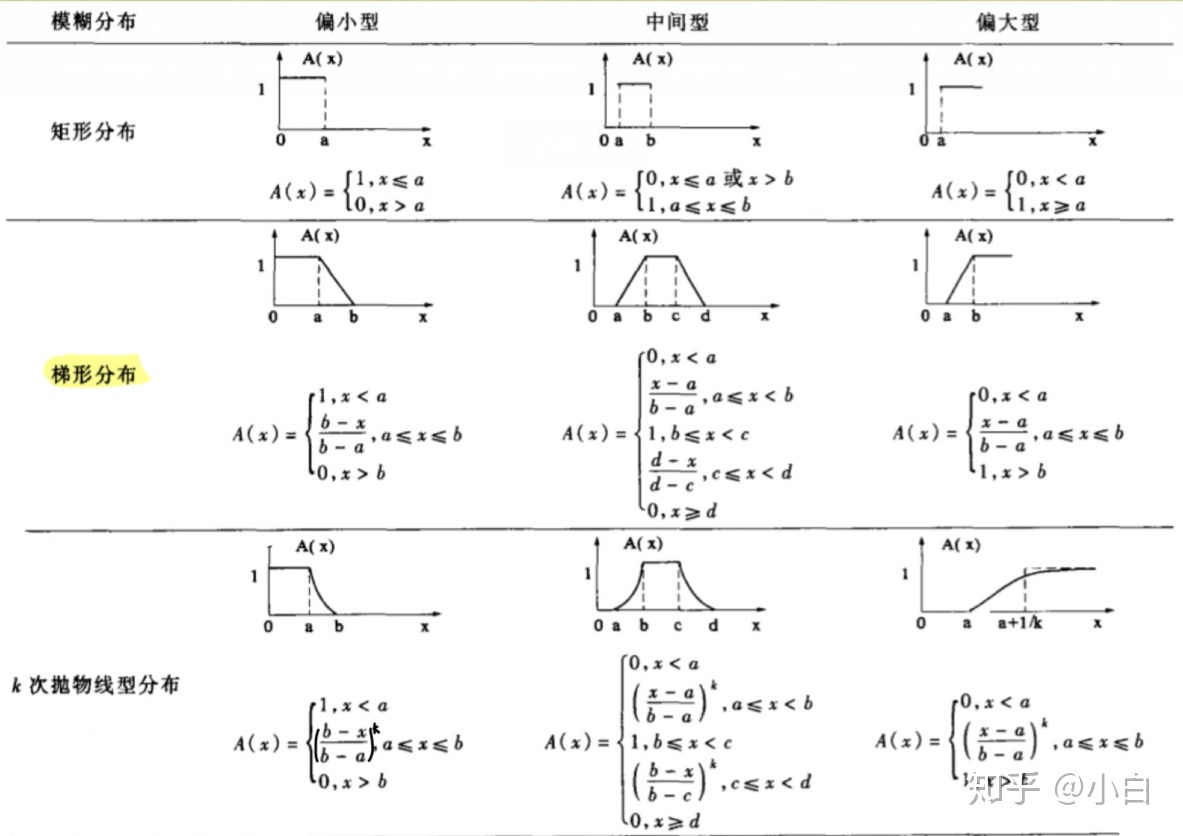
\includegraphics[scale=0.4]{Blurred Math1.jpg}
	\label{fig:label}
\end{figure}
\begin{figure}[h]
	\centering
	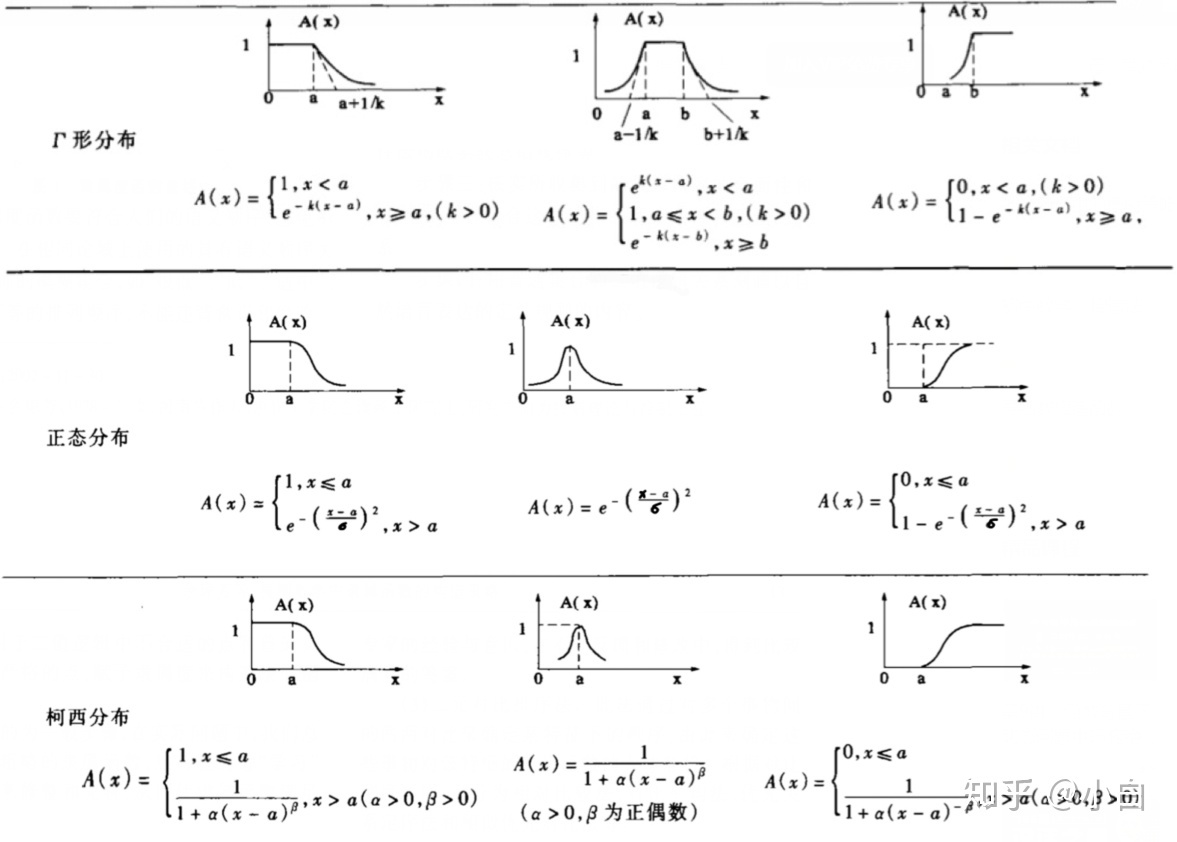
\includegraphics[scale=0.4]{Blurred Math2.jpg}
	\label{fig:label}
\end{figure}

隶属函数的确定方式有三种:模糊统计法;借助已有的客观尺度(如恩格尔系数);指派法。其中数学建模比赛中用得较多的为指派法:即凭主观意愿,在确定模糊集合的所属分类后,给它指派一个隶属函数,得到元素的隶属度。在实际建模比赛中,为了计算方便,最常使用的是\textbf{梯形分布式隶属函数。}\\
\indent\setlength{\parindent}{2em}对于偏小型模糊集合,隶属函数总体上递减,也就是元素的某个特征越大,隶属度越小;对于偏大型集合,隶属函数总体上递增,也就是元素的某个特征越大,隶属度越大;对于中间型集合,隶属函数总体上先递增后递减,中间一部分或是某个点取到最大值。\\
\textbf{对于一集模糊综合评价而言,确立方法如下:}\\
(1)确定因素集$U=\{u_1,...,u_n\}$,即确定评价指标(绩点、学工、科研)\\
(2)确定各因素的权重$A=\{a_1,...,a_n\}$,通过熵权法/TOPSIS/AHP等等\\
(3)确定评语集$V=\{v_1,...,v_m\}$,即给出相应的\textbf{模糊评语}如:优秀、良好、合格。\\
(4)确定模糊综合评价矩阵。举例:如果A同学GPA为3.89,\textbf{那么根据隶属函数$A(x)$来看},可能从「绩点」这个指标看,他相对于“优秀”的隶属度为0.9,相对于“良好”的隶属度为0.5,相当于“合格”的隶属度为0.1。那么A同学在绩点这一指标\textbf{相对于评语集$\boldsymbol{V}$的隶属向量$\boldsymbol{u_1}$为$\boldsymbol{u_1=[0.9,0.5,0.1]^T}$}
那么模糊综合评价矩阵可以写成$M_{3\times3}=[u_1,u_2,u_3]$\\
(5)进行综合评判。对于模糊综合评价矩阵$M$,任何一个元素$m_{ij}$代表着第$u_i$个指标的第$v_j$个评语。那么用矩阵乘法表示\textbf{所有评语$v_i$的综合隶属度向量B}:
\begin{equation*}
	\boldsymbol{B=AR}
\end{equation*}
容易知道$\boldsymbol{B}$是一个$1\times m$矩阵,每一个元素$b_j$都代表评语$v_j$的综合隶属度。那么,\textbf{最合适的评语就是隶属度最大的那个。}\\

\noindent \textbf{对于$n$级模糊综合评价,大致的思路是降维:\\
a.先得到第$n$层的判断矩阵\\
b.算出第$n$层的综合隶属度向量$B_n$\\
c.然后用第$n$层的综合隶属度向量组成第$n-1$层的判断矩阵,\\
d.算出第$n-1$层的综合隶属度向量$B_{n-1}$\\
e.然后用第$n-1$层的综合隶属度向量组成第$n-2$层的判断矩阵,\\
f.算出第$n-2$层的综合隶属度向量$B_{n-2}$\\
g.以此类推,得到第$1$层指标的综合隶属度向量,进而选择最合适的评语\\}
\newpage




\section{回归与分类问题}
\subsection{插值与拟合}
什么是插值
什么是拟合
拟合效果:用$\mathrm{R}^2$评价比较多
\subsection{回归分析}
包括一元线性回归与多元线性回归,注意掌握完整环节,不要求解方程放在那里就完事了,要做显著性检验,残差,画表格,用SPSSPro简单实现。\\
\indent\setlength{\parindent}{2em}一般来说,线性回归都可以通过最小二乘法或梯度下降法求出其方程。由于影响 y 的因素往往不止一个,假设有$x_1,x_2,...,x_k$,k 个因素,通常可考虑如下的线性关系式:\\
\begin{equation*}
	y=\omega_0+\omega_1x_1+...+\omega_nx_n
\end{equation*}
接下来简述用最小二乘法求$\hat \omega_i$的方式:\\
(0)首先,我们的目标是让RSS$\ =\sum\limits_{i}^{n}(y_i-\hat y_i)^2$最小,把它写成矩阵的形式会更为简便。\\
(1)构造权重向量:
$\omega=\begin{bmatrix}
	\omega_0\\
	...\\
	\omega_n\\
\end{bmatrix}$,特征向量
$x=\begin{bmatrix}
	1\\
	x_1\\
	...\\
	x_n\\
\end{bmatrix}$,
则多元函数可以写成$y=\omega^Tx$.\\
(2)构造$m\times n$的样本矩阵:
$X=\begin{bmatrix}
	1 & x_1^{(1)} & ... & x_n^{(1)}\\
	... & ... & ... &...\\
	1 & x_1^{(m)} & ... & x_n^{(m)}
\end{bmatrix}$,那么预测值向量$\hat y$可以这样得到:\\
\begin{equation*}
	X\omega=\begin{bmatrix}
		1 & x_1^{(1)} & ... & x_n^{(1)}\\
		... & ... & ... &...\\
		1 & x_1^{(m)} & ... & x_n^{(m)}
	\end{bmatrix}
	\begin{bmatrix}
		\omega_0\\
		...\\
		\omega_n\\
	\end{bmatrix}
	=\begin{bmatrix}
		\hat y_0\\
		...\\
		\hat y_n\\
	\end{bmatrix}
\end{equation*}
(3)由于$x^Tx=\sum\limits_{i=1}^{n}x_i^2$,损失函数可以表达为矩阵形式:
\begin{equation*}
	RSS=L(\omega)=||X\omega - y||^2
\end{equation*}
(4)求解矩阵的具体运算略过,我们可以对$RSS=L(\omega)$求$\omega$偏导计算得到:当$\L(\omega)$最小时,
\begin{equation*}
	\omega=(X^TX)^{-1}X^T y
\end{equation*}
(5)模型评估:除了RSS(最小残差平方和)之外,R$^2$也可以用于评估模型。R$^2$是预测结果与实际结果之间相关性的平方:
\begin{equation*}
	\mathrm{R}^2=1-\dfrac{\mathrm{RSS}}{\mathrm{TSS}}
\end{equation*}
其中
\begin{equation*}
	RSS =\sum\limits_{i}^{n}(y_i-\hat y_i)^2
	,\quad
	TSS=\sum\limits_{i}^{n} (y_i-\bar y_i)^2
\end{equation*}

\subsection{因子分析(探索性)}
\indent\setlength{\parindent}{2em}因子分析是基于降维的思想,在尽可能不损失或者少损失原始数据信息的情况下,将错综复杂的众多变量聚合成少数几个独立的公共因子,这几个公共因子可以反映原来众多变量的主要信息,在减少变量个数的同时,又反映了变量之间的内在联系。\\
\indent\setlength{\parindent}{2em}举个简单的例子:因子分析法可以通过分析数据间的关联性,将「语文、数学、英语、物理、化学、生物、地理、历史、政治、信息」这些变量降维成「文科、理科、语言学」三个变量。\\
\indent\setlength{\parindent}{2em}通常因子分析有三种作用:一是用于因子降维,二是计算因子权重,三是计算加权计算因子汇总综合得分。\\
\indent\setlength{\parindent}{2em}因子分析可以通过SPSSPro实现,下面解读一下各参数的意义:\\
\noindent(1)首先进行KMO和Bartlett的检验,判断是否可以进行因子分析。对于KMO值:\textbf{0.9上非常合适做因子分析,0.7-0.9之间适合,0.6-0.7之间尚可,0.5-0.6之间表示差,0.5下应该放弃;通KMO值检验可以说明是否适合使用因子分析。}对于Bartlett的检验,\textbf{若(P<0.05),}拒绝原假设,\textbf{则说明可以做因子分析},若不拒绝原假设,则说明这些变量可能独立提供一些信息,不适合做因子分析。\\

\noindent(2)我们怎么知道需要多少个主因子?\textbf{通过分析方差解释表格和碎石图,确定因子的数量。 }\textbf{方差解释表格主要是看因子对于变量解释的贡献率}(可以理解为究竟需要多少因子才能把变量表达为100$\%$),如果太低(如低于60$\%$)则需要调整因子数据。 \textbf{一般情况下,方差解释率越高,说明该主成分越重要,权重占比也应该越高。}旋转后因子的方差解释率,特征根,方差解释率,累积方差解释率,用于求解主成分公式。 当因子数量设置为1时,单个因子的方差解释率不支持旋转,因此旋转后方差解释率为空。\textbf{碎石图的作用是根据特征值下降的坡度来确认需要选择的因子个数},在下降平缓的肘部即为选择的因子个数。这两者结合可用于确认或调整因子个数。\\

\noindent(3)\textbf{通过分析因子载荷系数与热力图,可以分析到每个因子中隐变量的重要性},如研究“多金属矿体”中25种有用元素的分布规律,其中各元素视为指标,假设前文确定得到5个因子,因子1中,$SO$、$SO_2$、$Na_2S$、$HS$、$H_2S$因子载荷系数较大,因此可将因子1确定为硫化物成分,以此类推,也可结合具体业务进行各因子的隐变量分析。\\

\noindent(4)通过分析成分矩阵,得出因子公式。\\

\noindent(5)通过分析成分矩阵,得出因子成分公式与权重。\\

\noindent(6)输出因子分析法综合得分。\\





\subsection{聚类分析(K-means)}
(对于F题要尤其关注)聚类分析及求解方法,例如某一个政策用于许多国家,要对国家进行分类。对样本进行分类称为Q型聚类分析,对指标进行分类称为R型聚类分析。\\
\indent\setlength{\parindent}{2em}K-means聚类步骤是一个循环迭代的算法:假定我们要对N个样本观测做聚类,要求聚为K类\\
(1)选择K个点作为初始中心点;\\
(2)接下来,按照距离初始中心点最小的原则,把所有观测分到各中心点所在的类中;\\
(3)每类中有若干个观测,计算K个类中所有样本点的均值,作为第二次迭代的K个中心点;\\
(4)然后根据这个中心重复第2、3步,直到收敛(中心点不再改变或达到指定的迭代次数),聚类过程结束。\\
\indent\setlength{\parindent}{2em}其中,(选择的经典的欧式)距离为$d(X,Y)=||X-Y||^2=\sqrt{(x_1-y_1)^2+...+(x_n-y_n)^2}$,我们记聚类中心为$C_i$,那么差异可以用误差平方和表示:$SSE=\sum\limits_{i=1}^{K} \sum\limits_{x\in C_i}(C_i-x)^2$\\
\indent\setlength{\parindent}{2em}关于K值怎么确定,虽然K设置得越大,样本划分得就越细,每个簇的聚合程度就越高,误差平方和SSE自然就越小。但到后面,SSE的下降幅度会小很多。这个时候往往用“手肘法”解决,当K小于样本真实簇数J时,K每增大一个单位,就会大幅增加每个簇的聚合程度,这时SSE的下降幅度会很大;当K接近J时,再增加K所得到的聚合程度回报会迅速变小,SSE的下降幅度也会减小;这个SSE-K曲线的拐点(手肘)就是理想的真实簇数。\\
\indent\setlength{\parindent}{2em}需要牢记一件事,初始中心点的选择非常重要。以及K-mean受离群值影响大。\\
\newpage
\section{预测模型}
\subsection{时间序列模型}
一些简单的模型,比如说:指数平滑,灰色模型,ARIMA等简单的预测模型就可以,甚至有时候线性回归就解决了。
对于F题,需要用到灰色预测模型。
\subsection{灰色预测模型GM(1,1)}
\indent\setlength{\parindent}{2em}白色系统的内部特征是完全已知的,给系统一个“输入”,就能得到一个准确的“输出”,整个过程是已知的。\\
\indent\setlength{\parindent}{2em}黑色系统是外界并不知道系统的内部信息,只能通过它与外界的联系来加以观测研究。\\
\indent\setlength{\parindent}{2em}灰色系统介于白色和黑色系统之间,一部分信息是已知的,另一部分信息是未知的,系统内各因素间有不确定的关系。\\
\indent\setlength{\parindent}{2em}举个例子:某城市1986到1992年道路噪声平均声级数据见下表,请预测下一年的数据。\\
\begin{table}[h]
	\centering
	\begin{tabular}{ccc}
		\hline
		年份& 噪声 \\
		\hline
		1986 & 71.1 \\
		1987 & 72.4\\
		1988 & 72.4\\
		1989 & 72.1\\
		1990 & 71.4\\
		1991 & 72.0\\
		1992 & 71.6\\
		\hline
	\end{tabular}
\end{table}

\indent\setlength{\parindent}{2em}“年份-噪声”就是一个灰色系统,年份和噪声之间存在联系(常识或从文献得知),但我们不知道具体的函数表达式,无法在数学上求解下一年的数据。该灰色系统的特点包括:\\
(1)数据量太少,无法用回归或神经网络预测(2)年份和噪声的数据是已知的(3)年份和噪声之间存在内在联系(4)具体函数关系未知(5)短期预测(只预测下一年)\\

\noindent 灰色预测模型是这样构建的:\\
(0)首先,序列适不适合做GM(1,1)建模?需要通过级比检验,定义参数:
\begin{equation*}
	\lambda(k)=\dfrac{x^{(0)}(k-1)}{x^{(0)}(k)}
\end{equation*}
如果$\lambda(k)$在区间$(e^{-\frac{2}{n+1}}, e^{-\frac{2}{n+2}})$内,说明可以用GM(1,1)模型。如果在区间外,那就必须通过平移变换才可能适用于GM(1,1)模型了:先给每个数据加上任意常数$c$,求解完以后再减去$c$\\

\noindent\textbf{(1)构造灰色预测模型:}要根据已有数据序列生成一个新的序列,常用方法有\textbf{累加生成,累减生成,加权邻值生成}。注意,已知年份和新序列的数据是已知的,我们现在缺少的是两者的函数关系式;一旦函数求出来了,代入下一年的年份,就能求出下一年的噪声预测值了。\\
\textbf{累加生成序列公式}:
\begin{equation*}
	x^{(1)}(t)=\sum_{i=1}^{t}x^{(0)}(i)
\end{equation*}
\noindent \textbf{均值生成序列公式:}
\begin{equation*}
	z^{(1)}(t)=\omega x^{(1)}(t)+(1-\omega )x^{(1)}(t-1)
\end{equation*}
其中常取$\omega=\dfrac{1}{2}$\\
\textbf{(2)对$x^{(1)}(t)$建立$x^{(1)}(t)$的一阶线性微分方程:}
\begin{equation*}
	\dfrac{\mathrm{d}x^{(1)}(t)}{\mathrm{d}t}+az^{(1)}(t)=b
\end{equation*}
\textbf{(3)对于这个白化方程}(将灰色系统化为白色系统),$a,b$两个参数是不知道的,这时候只能通过\textbf{最小二乘法},通过最小化误差的平方和求得最佳的参数$a,b$。
求解可以用矩阵表示:记
\begin{equation*}
	Y=\begin{bmatrix}
		x^{(0)}(2)\\
		x^{(0)}(3)\\
		...\\
		x^{(0)}(n)\\
	\end{bmatrix},
	B=\begin{bmatrix}
		-z^{(1)}(2) & 1\\
		-z^{(1)}(3) & 1\\
		...\\
		-z^{(1)}(n) & 1\\
	\end{bmatrix},U=
\begin{bmatrix}
	a\\
	b\\
\end{bmatrix}
\end{equation*}
最小二乘法也就是求$(Y-BU)^T(Y-BU)$取最小值时的$U$,求解其估计值为:
\begin{equation*}
	\hat U= \begin{bmatrix}
		\hat a \\
		\hat b \\
	\end{bmatrix}=(B^TB)^{-1}B^TY
\end{equation*}
这样就得到了未知参数$a,b$的估计值。\\
\textbf{(4)这个一阶线性微分方程的方程解是:}
\begin{equation*}
	\hat x^{(1)}(t+1)=(x^{(0)}(1)-\dfrac{\hat b}{\hat a})\cdot e^{-\hat a t}+\dfrac{\hat b}{\hat a}
\end{equation*}
代入刚刚求得的$a,b$即可。由上面的公式同样可以还原出原始值
\begin{equation*}
	\hat x^{(0)}(t+1)=(1-e^{\hat a})(x^{(0)}(1)-\dfrac{\hat b}{\hat a})\cdot e^{-\hat a t}
\end{equation*}
\textbf{(5)残差检验:}常用后验差比值$C$来衡量,计算公式如下:
定义
\begin{equation*}
e(k)=X^{(0)}(k)-\hat X^{(0)}(k),\quad \bar X^{(0)}(k)=\dfrac{1}{n}\sum_{i=1}^{n}X^{(0)}(i),\quad \bar e=\dfrac{1}{n}\sum_{i=1}^{n}e(i)
\end{equation*}
\begin{equation*}
	S_1^2=\dfrac{1}{n}\sum_{i=1}^{n}(X^{(0)}(i)-\bar X^{(0)}(i))^2
\end{equation*}
\begin{equation*}
	S_2^2=\dfrac{1}{n}\sum_{i=1}^{n}(e(i)-\bar e)^2
\end{equation*}
则后验差比$C=\dfrac{S_2}{S_1}$
如何评判这个灰色预测模型的精度呢?如表所示:
\begin{table}[h]
	\centering
	\begin{tabular}{ccc}
		\hline
		模型精度等级& 后验方差比值C \\
		\hline
		好 & $C \le 0.35$\\
		合格 & $0.35<C\le 0.50$\\
		勉强 & $0.5<C \le 0.65$\\
		不合格 & $C>0.65$\\
		\hline
	\end{tabular}
\end{table}\\
总结一下模型的优缺点:在数据少且无明显规律时,利用微分方程可以挖掘数据本质规律,但灰色预测只适合短期预测,\textbf{指数增长的预测:比如人口/游客数量/灾变预测/天气预测等等。}
\subsection{道路交通事故Verhulst模型}
\textbf{在实际问题中,常遇到原始数据本身呈 S 形的过程,}这时,可取原始数据为 $x^{(1)}$ ,其一次累减生成(1—IAGO)为$x^{(0)}$ ,建立 Verhulst 模型。与灰色预测模型GM(1,1)非常类似,唯一的差别在于处理数据和确定白化方程的几步。(但在SPSSPro没有Verhulst模型的选项)\\
(1)第一步:对原始序列$x^{(1)}(t)$做一次累减生成,公式如下
\begin{equation*}
	x^{(0)}(t)=x^{(1)}(t)-x^{(1)}(t-1), \quad t=2,3,...
\end{equation*}
(2)第二步:再对$x^{(1)}(t)$做紧邻均值生成,公式如下:
\begin{equation*}
	z^{(1)}(t)=\omega x^{(1)}(t)+(1-\omega )x^{(1)}(t-1)
\end{equation*}
其中常取$\omega=\dfrac{1}{2}$\\
(3)记
\begin{equation*}
	Y=\begin{bmatrix}
		x^{(0)}(2)\\
		x^{(0)}(3)\\
		...\\
		x^{(0)}(n)\\
	\end{bmatrix},
	B=\begin{bmatrix}
		-z^{(1)}(2) &(z^{(1)}(2))^2\\
		-z^{(1)}(3) & (z^{(1)}(3))^2\\
		...\\
		-z^{(1)}(n) & (z^{(1)}(n))^2\\
	\end{bmatrix},U=
	\begin{bmatrix}
		a\\
		b\\
	\end{bmatrix}
\end{equation*}并对对参数列$ U= \begin{bmatrix}
	 a \\
	 b \\
\end{bmatrix}$作最小二乘分析。\\
(4)白化方程是最重要的一步:Verhulst模型的微分方程为:
\begin{equation*}
	\dfrac{\mathrm{d}x^{(1)}(t)}{\mathrm{d}t}+az^{(1)}(t)=b(x^{(1)}(t))^2
\end{equation*}
可以求解得到Verhulst模型的时间响应序列为
\begin{equation*}
	\hat x^{(1)}(t+1)=\dfrac{\hat ax^{(1)}(1))}{\hat bx^{(1)}(1)+(\hat a -\hat b x^{(1)}(1))\cdot e^{\hat at}}
\end{equation*}
(5)最后进行残差检验.\\
\subsection{马尔可夫链}
随机变量$X$在${X_1,...X_n,X_{n+1},...}$中取值,如果下一个状态$X_{n+1}$只取决于上一个状态$X_n$,那么称这个序列$\{X_n\}$为马尔可夫链。令$P_{ij}=P(X_{n+1}=j|X_n=i)$,这样一来,整个序列$\{X_n\}$将来的性质(指概率值)都会被$p_{ij}$和$X_i$的初始值确定。\\
\indent\setlength{\parindent}{2em}从定义可以看出,马尔可夫链是离散的。$p_{ij}$可以更通俗地理解为从序列中的第$i$个到第$j$个的概率,通过转移状态图可以画出转移状态矩阵:
\begin{equation*}
	\begin{bmatrix}
		p_{11}&p_{12}&...&p_{1n} \\
		p_{21}&p_{22}&...&p_{2n} \\
		...&...&...&...\\
		p_{n1}&p_{n2}&...&p_{nn}
	\end{bmatrix}
\end{equation*}
每运动一次,就将初始状态矩阵乘以转移状态矩阵,对应的$p_{ij}$概率值就会出现在$(i,j)$的位置。例如:\\
\begin{equation*}
	\begin{bmatrix}
		p_{01}&p_{02}&...&p_{0n} \\
	\end{bmatrix}
	\begin{bmatrix}
		p_{11}&p_{12}&...&p_{1n} \\
		p_{21}&p_{22}&...&p_{2n} \\
		...&...&...&...\\
		p_{n1}&p_{n2}&...&p_{nn}
	\end{bmatrix}
\end{equation*}
我们记
$\begin{bmatrix}
	p_{01}&p_{02}&...&p_{0n} \\
\end{bmatrix}=\pi_{n+1}$,转移状态矩阵为$P$,则每一次从$X_{n}$到$X_{n+1}$的运动都可以记为
\begin{equation*}
	\pi_{n+1}=\pi_n\cdot P
\end{equation*}

马尔可夫链有一个「稳定状态分布」的性质:对于遍历的马尔可夫链,当$n$充分大时,对$X_n$状态的矩阵乘以转移状态矩阵后,第$X_{n+1}$状态的矩阵的每个元素都趋于一个确定的值。(当然,也存在周期的马尔可夫链,这时候$X_i$状态的矩阵的元素就会周期性跳跃出现)我们关心这个极限值是多少,只需要求解一个\textbf{n元一次}方程组$\pi=\pi\cdot P$,其中$\pi$是$n \to \infty$的状态矩阵$\begin{bmatrix}
	p_{\infty1}&p_{\infty2}&...&p_{\infty n} \\
\end{bmatrix}$。
\subsection{马尔可夫过程}
马尔可夫链描述离散过程,而马尔可夫过程描述连续过程。
\subsection{指数平滑}
一般说来历史数据对未来值的影响是随时间 间隔的增长而递减的。所以,更切合实际的方法应是对各期观测值依时间顺序进行加权 平均作为预测值。指数平滑法可满足这一要求,而且具有简单的递推形式。指数平滑法根据平滑次数的不同,又分为一次指数平滑法、二次指数平滑法和三 次指数平滑法等。\\
\indent\setlength{\parindent}{2em}\textbf{对于一次指数平滑而言:}
设时间序列为$y_1,...,y_t,...$,加权系数为$\alpha \in (0,1)$,那么一次指数平滑为:
\begin{equation*}
	S_t^{(1)}=\alpha y_t+(1-\alpha)S_{t-1}^{(1)}=S_{t-1}^{(1)}+\alpha(y_t-S_{t-1}^{(1)})
\end{equation*}
将这个递推式展开,就能注意到
\begin{equation*}
S_t^{(1)}=\alpha y_t+(1-\alpha)S_{t-1}^{(1)}=\alpha y_t+(1-\alpha)(\alpha y_{t-1}+(1-\alpha)S_{t-2}^{(1)})=...=\alpha \sum_{j=0}^{\infty}(1-\alpha)^j y_{t-j}
\end{equation*}
这表明$S_t^{(1)}$是全部历史数据的加权平均,加权系数为$\alpha(1-\alpha)^j$,这些加权系数等比数列求和为1,因此称之为「指数平滑」。\\
我们令$\hat y_{t+1}=S_t^{(1)}$,立刻得到$\hat y_{t+1}=\alpha y_t+(1-\alpha)\hat y_{t}$,这告诉我们第t+1期预测值是以“第t期指数平滑值“为基础计算的。
对于加权系数$\alpha$,从两方面理解:
\begin{equation*}
\hat y_{t+1}=\alpha y_t+(1-\alpha)\hat y_{t}
\end{equation*}
体现的是“新预测值中新数据与原预测值占的权重。”$\alpha$越大,新数据所占的权重越大,$\alpha$越小,原预测值所占的比重越大。另一方面,
\begin{equation*}
	\hat y_{t+1}=\hat y_{t}+\alpha(y_t-\hat y_t)
\end{equation*}
体现的是“新预测值根据预测误差对原预测值修正得到的”,$\alpha$越大,修正幅度越大。$\alpha$的选取可以依照下面的原则:\\
\begin{table}[h]
	\centering
	\begin{tabular}{ccc}
		\hline
		$\alpha$值& 情况 \\
		\hline
		0.1~0.5 & 时间序列波动不大、比较平稳\\
		0.6~0.8 & 时间序列有迅速且明显的变动倾向\\
		\hline
	\end{tabular}
\end{table}

\noindent 除了$\alpha$的选取以外,还要确定合适的初始值$s_0^{(1)}$:
\begin{table}[h]
	\centering
	\begin{tabular}{ccc}
		\hline
		$s_0^{(1)}$值& 情况 \\
		\hline
		可选取第一期数值 & 时间序列的数据较多(20个以上)\\
		最初几期实际值的平均值 & 时间序列的数据较少(20个以下)\\
		\hline
	\end{tabular}
\end{table}

\indent\setlength{\parindent}{2em}当时间序列的变动出现直线趋 势时,用一次指数平滑法进行预测,仍存在明显的滞后偏差。因此,也必须加以修正。 修正的方法与趋势移动平均法相同,即再作二次指数平滑,利用滞后偏差的规律建立直线趋势模型。\\
\indent\setlength{\parindent}{2em}\textbf{对于二次指数平滑而言:设}
\begin{equation*}
	S_t^{(1)}=\alpha y_t+(1-\alpha)S_{t-1}^{(1)}
\end{equation*}
\begin{equation*}
	S_t^{(2)}=\alpha S_t^{(1)}+(1-\alpha)S_{t-1}^{(2)}
\end{equation*}
其中$S_t^{(1)}$为一次指数的平滑值,$S_t^{(2)}$为二次指数的平滑值。接着使用直线趋势模型进行预测:\\
\begin{equation*}
\hat y_{t+m}=a_t+b_t m, \quad m=1,2,...
\end{equation*}
\begin{equation*}
\begin{cases}
a_t=2S_t^{(1)}-S_t^{(2)}\\
b_t=\dfrac{\alpha}{1-\alpha}(S_t^{(1)}-S_t^{(2)})
\end{cases}
\end{equation*}

\indent\setlength{\parindent}{2em}当时间序列的变动表现为二次曲线趋势时,则需要用三次指数平滑法。三次指数平滑是在二次指数平滑的基础上,再进行一次平滑。
\indent\setlength{\parindent}{2em}\textbf{对于三次指数平滑而言:}
\begin{equation*}
	S_t^{(1)}=\alpha y_t+(1-\alpha)S_{t-1}^{(1)}
\end{equation*}
\begin{equation*}
	S_t^{(2)}=\alpha S_t^{(1)}+(1-\alpha)S_{t-1}^{(2)}
\end{equation*}
\begin{equation*}
	S_t^{(3)}=\alpha S_t^{(2)}+(1-\alpha)S_{t-1}^{(3)}
\end{equation*}
其中$S_t^{(3)}$为三次指数平滑值。接着使用二次函数预测模型:\\
\begin{equation*}
	\hat y_{t+m}=a_t+b_t m+c_t m^2, \quad m=1,2,...
\end{equation*}
\begin{equation*}
	\begin{cases}
		a_t=3S_t^{(1)}-3S_t^{(2)}+S_t^{(3)}\\
		b_t=\dfrac{\alpha}{2(1-\alpha)^2}((6-5\alpha)S_t^{(1)}-2(5-4\alpha)S_t^{(2)}+(4-3\alpha)S_t^{(3)})\\
		c_t=\dfrac{\alpha^2}{2(1-\alpha)^2}(S_t^{(1)}-2S_t^{(2)}+S_t^{(3)})
	\end{cases}
\end{equation*}



\newpage
\section{图论算法}
\subsection{邻接矩阵}
\noindent \textbf{1.邻接矩阵:}由两方面组成:对于一个图$G=(V,E)$
\begin{itemize}
	\item 建立一个顶点表(一维数组)\mintinline{C}|Vexs[n]|,记录图$G$的各个顶点信息$v_1,...,v_n$。
	\item 建立一个邻接矩阵(二维数组)\mintinline{C}|G->arcs[n][n]|,定义为
	\begin{equation*}
		\mintinline{C}|G->arcs[n][n]|=\begin{cases}
			1 & \left\langle i,j \right\rangle \in E \ \mathrm{or} \ (i,j)\in E\\
			0 & \mathrm{otherwise}
		\end{cases}
	\end{equation*}
	特别的,网的邻接矩阵可以定义为
	\begin{equation*}
		\mintinline{C}|G->arcs[n][n]|=\begin{cases}
			w_{ij} & \left\langle i,j \right\rangle \in E \ \mathrm{or} \ (i,j)\in E\\
			\infty & \mathrm{otherwise}
		\end{cases}
	\end{equation*}
	其中$w_{ij}$为边/弧$e_{ij}$的权值。
\end{itemize}

\subsection{迪杰斯特拉算法(Dijkstra)}
\begin{enumerate}
	\item \textbf{将所有顶点的集合$V$分类:}$V=S+T$,其中:
	\begin{enumerate}
		\item $S$:已求出最短路径的顶点的集合
		\item $T$:尚未确定最短路径的顶点集合
	\end{enumerate}
	\item \textbf{初始化:}令源点$v_0\in S$,先找出从$v_0$到各顶点$v_k$的直达路径$(v_0,v_k),k=1,2,...,n$。
	\item \textbf{选择:}从这些路径中找出一条长度最短的路径$(v_0,v_i)$,随后将$v_i$由$T$加入$S$。
	\item \textbf{更新:}固定住$(v_0,v_i)$作为\textbf{源点$v_0$到顶点$v_i$的最短路径},对\textbf{其余}各条路径进行适当调整:
	\begin{enumerate}
		\item 如果图中存在弧$(v_i,v_k)$,且$(v_0,v_i)+(v_i,v_k)<(v_0,v_k)$,则用弧$(v_0,v_i,v_k)$替代$(v_0,v_k)$。\\
		(意义:用新加入$S$的$v_i$来更新路径,使路径更短。)
	\end{enumerate}
	\item \textbf{在调整后的各条路径中,重复步骤3、4,以此类推,直到所有的顶点都加入$S$}。
\end{enumerate}
以下面这个有向网$G$演示Dijkstra算法的运行模式:
\begin{center}
	\begin{figure}[h]
		\centering
		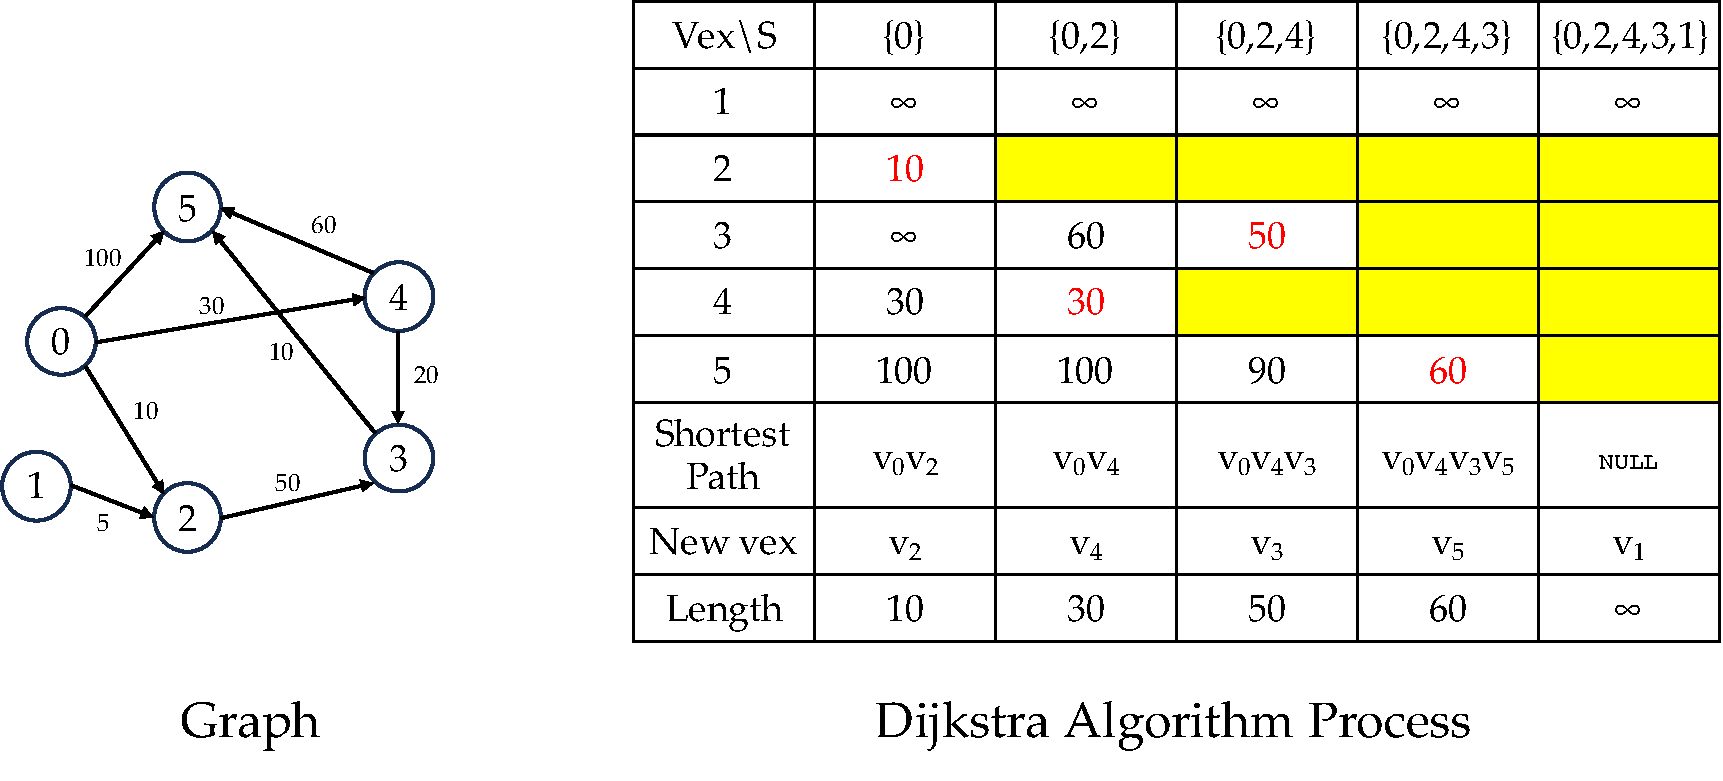
\includegraphics[scale=0.53]{Dijkstra.pdf}
	\end{figure}
\end{center}
{\kaishu \textbf{时间复杂度分析:}}$O(n^2)$\\


\subsection{弗洛伊德算法(Floyd)}
\begin{enumerate}
	\item 对于$n$个顶点,置其\textbf{邻接矩阵}和对应的\textbf{路径矩阵}。
	\begin{enumerate}
		\item 邻接矩阵$AM$:对角线元素为0,若存在弧$(v_i,v_j)$,则$AM_{ij}$为权值;否则$AM_{ij}$为$\infty$
		\item 路径矩阵$PM$:对角线元素为空,若存在弧$(v_i,v_j)$,则在$PM_{ij}$中记$v_iv_j$;否则$PM_{ij}$为空
	\end{enumerate}
	\item 对原直接路径中增加中间顶点$v_k$:
	\begin{enumerate}
		\item 如果增加$v_k$后路径变短,则修改邻接矩阵$AM_{ij}$处的值为新的路径长度,修改路径矩阵$PM_{ij}$处为$v_iv_kv_j$。
		\item 否则维持邻接矩阵的原值和路径矩阵的原路径。
	\end{enumerate}
\end{enumerate}
以下面这个有向网$G$演示Floyd算法的运行模式:
\begin{center}
	\begin{figure}[h]
		\centering
		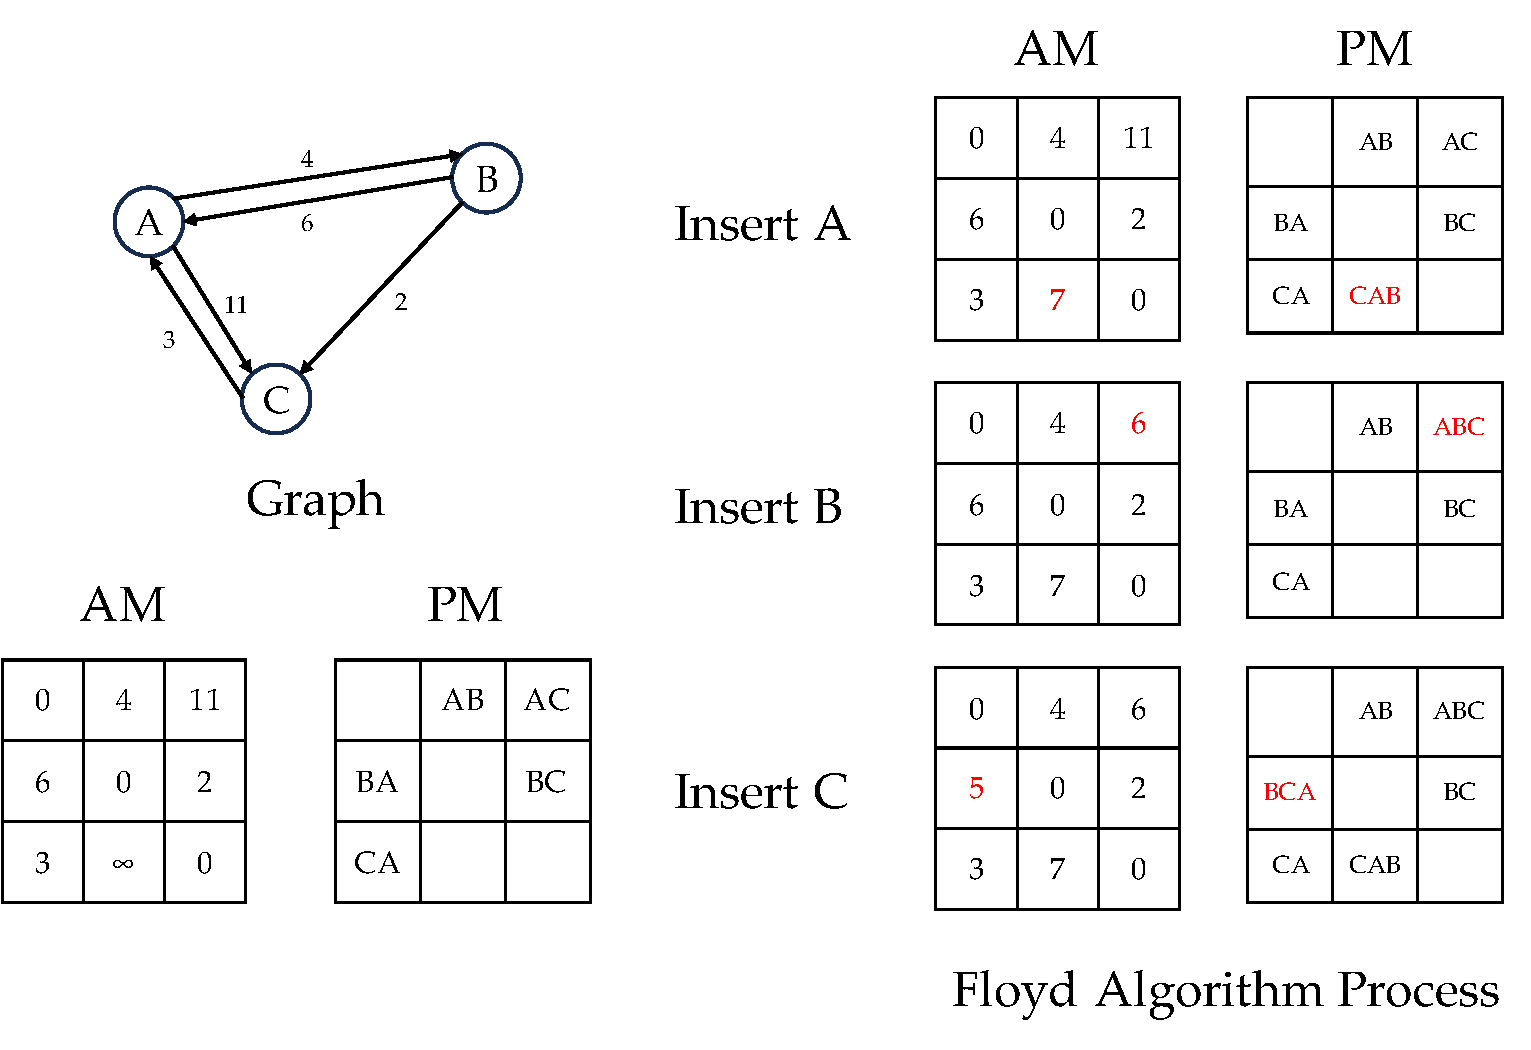
\includegraphics[scale=0.5]{Floyd.pdf}
	\end{figure}
\end{center}
{\kaishu \textbf{时间复杂度分析:}}$O(n^3)$


\section{数据分析}
首先要知道统计量:标准差、方差、极差、偏度、峰度
了解正态分布,卡方分布,t分布,F分布
(对于F题)方差分析很重要
\section{交叉学科领域知识}
\subsection{系统动力学}
分析指标体系内各个指标的影响机理,求解软件是Vensim。
事实上,只要Vensim花一个图,提到自己用了系统动力学分析即可。
\subsection{运筹学}
看清华大学出版社《运筹学 第4版》,只要符合理论的正确的规划模型,哪怕不会求解,只要合理的答案编出来就好。
\section{美赛建模里的数据问题}
对于未给定数据的题,当数据很难找时,怎么编数据?

\end{document}